% "{'classe':('PSI'),'chapitre':'dyn_pfd','type':('application'),'titre':'Kart', 'source':'C. Gamelon et P. Dubois','comp':('C1-05','C2-09'),'corrige':False}"
%\setchapterimage{bandeau}
\chapter*{Application \arabic{cptApplication} \\ 
Kart -- \ifprof Corrigé \else Sujet \fi}
\addcontentsline{toc}{section}{Application \arabic{cptApplication} : Kart -- \ifprof Corrigé \else Sujet \fi}

\iflivret \stepcounter{cptApplication} \else
\ifprof  \stepcounter{cptApplication} \else \fi
\fi

\setcounter{question}{0}
\marginnote{C. Gamelon \& P. Dubois.}
\marginnote[1cm]{
\UPSTIcompetence[2]{C1-05}
\UPSTIcompetence[2]{C2-09}
}
\begin{marginfigure}[3cm]
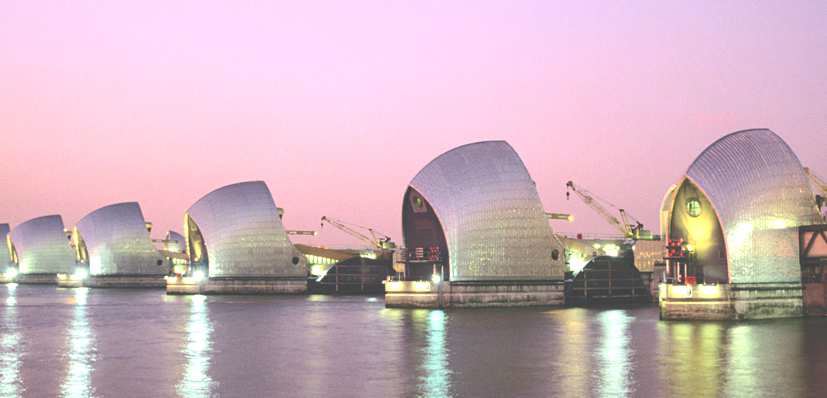
\includegraphics[width=\linewidth]{fig_00}
\end{marginfigure}




\ifprof
\else

\begin{marginfigure}[6cm]
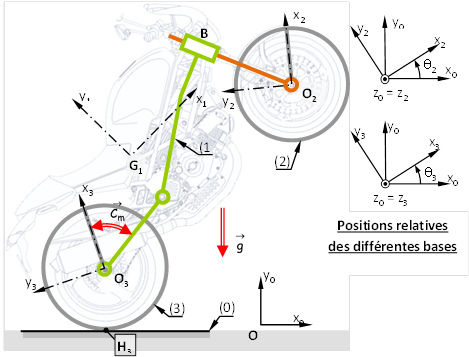
\includegraphics[width=\linewidth]{fig_01}
\end{marginfigure}

Au démarrage, le kart est bridé au sol. Le démarreur électrique exerce un couple de $C_m = \SI{1}{N.m}$ sur le vilebrequin et lorsque la vitesse de rotation atteint \SI{1200}{tr/min}, la combustion du mélange air essence commence et le moteur thermique démarre. Dans cette phase de démarrage l’embrayage est ouvert et ne transmet pas de mouvement.
Le vilebrequin est guidé en rotation par rapport au carter moteur. Ce guidage est modélisé par une liaison rotule en $O$ et linéaire annulaire en $B$ d’axe $\axe{O}{z}$. $\vect{OB}=a\vect{z}$.


\begin{marginfigure}[8cm]
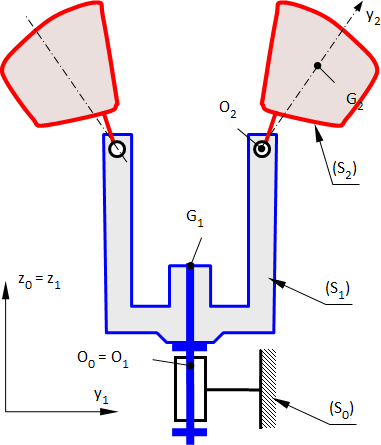
\includegraphics[width=\linewidth]{fig_02}
\end{marginfigure}

Le vilebrequin est de masse $m_2$ et de centre de gravité $G_2$ avec $\vect{OG_2}=l_2\vect{z}$. On a : $\inertie{G_2}{2}=\matinertie{A}{B}{C}{-D}{0}{0}{\mathcal{R}_2}$.


\question{Faire un graphe de liaison correspondant à la situation de démarrage.}

\question{Déterminer le temps de démarrage du moteur (équation du mouvement) et les actions dans le guidage en rotation.}

Nouvelle situation de démarrage : le kart de masse $m_1$ et centre inertie $G_1$ n’est plus bridé et peut de déplacer horizontalement. $\vect{O_0 G_1}=\lambda \vect{x}+h\vect{y}$ et $\vect{OG_1}=b\vect{y}$.

\question{Faire un graphe de liaison correspondant à la nouvelle situation de démarrage.}

\question{Déterminer les déplacements du kart au démarrage.}

\question{Identifier les modifications des résultats si $\vect{OG_2}=l_2\vect{z}+e\vect{y_2}$.}




\fi

\ifprof
\begin{center}
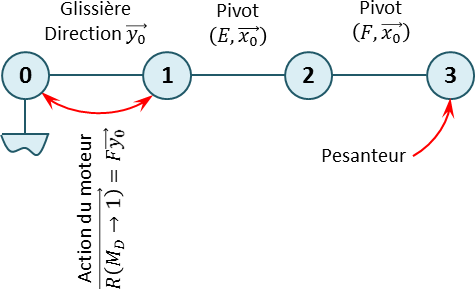
\includegraphics[width=.75\linewidth]{cor_01}
\end{center}

\begin{center}
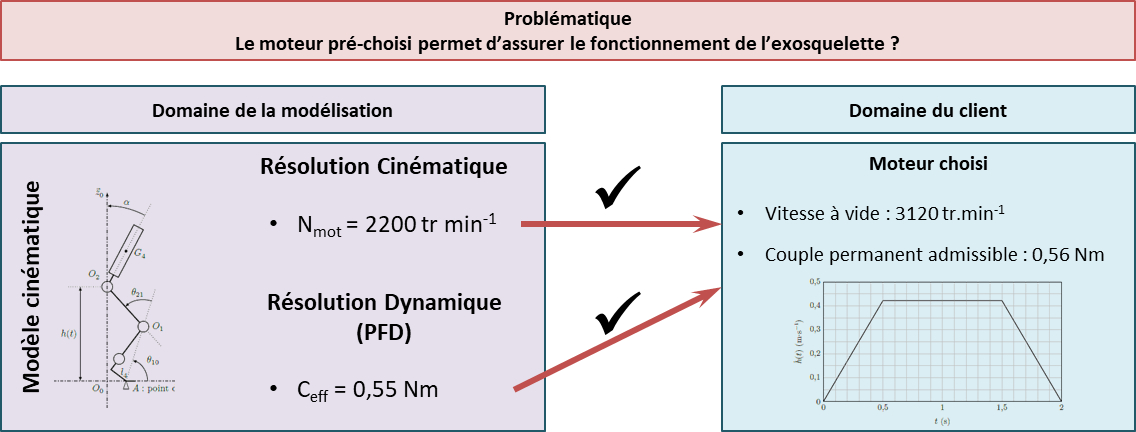
\includegraphics[width=.75\linewidth]{cor_02}
\end{center}
\else
\fi
%
%\textbf{On isole le solide \textbf{(1)}.}
%
%\textbf{On réalise le bilan des actions mécaniques.}
%\begin{itemize}
%\item Liaison pivot : $\torseurstat{T}{0}{1}
%=\torseurl{X_{01}\vect{x_0}+Y_{01}\vect{y_0}+Z_{01}\vect{z_0}}{M_{01}\vect{y_0}+N_{01}\vect{z_0}}{O}
%=\torseurl{Y_{01}\vect{y_0}+Z_{01}\vect{z_0}}{\vect{0}}{O}$.
%\item Liaison ponctuelle : $\torseurstat{T}{2}{1}
%=\torseurl{Y_{21}\vect{y_0}+Z_{21}\vect{z_0}}{\vect{0}}{I}$. On a $Z_{21}<0$, $Y_{21}>0$ et à la limite du glissement, $Y_{21}=-fZ_{21}$. 
%
%$\vectm{O}{2}{1}=\vectm{I}{2}{1}+\vect{OI}\wedge \vectf{2}{1}=\left( e\vect{z_1}+R\vect{z_0}\right)\wedge \left(Y_{21}\vect{y_0}+Z_{21}\vect{z_0} \right)$ 
%$= -eY_{21}\cos\theta \vect{x_0}-e Z_{21}\sin\theta\vect{x_0}-RY_{21}\vect{x_0}$
%$= -\left(\left(e\cos\theta+R\right)Y_{21} +e Z_{21}\sin\theta\right)\vect{x_0}$.
%
%\item Couple moteur : $\torseurstat{T}{\text{Moteur}}{1}
%=\torseurl{\vect{0}}{C_m\vect{x_0}}{O}$.
%\end{itemize}
%
%\textbf{Calcul de $\vectmd{O}{1}{0}\cdot \vect{x_0}$.}
% 
%$O$ est un point fixe et $I_1$ moment d'inertie par rapport à $\axe{O}{x_0}$ on a donc : 
%$\vectmd{O}{1}{0}\cdot \vect{x_0}
%=\left[\dfrac{\dd \vectmc{O}{1}{0}}{\dd t}\right]_{\mathcal{R}_0}\vect{x_0}
%=\left[\dfrac{\dd \vectmc{O}{1}{0}\cdot \vect{x_0}}{\dd t}  \right]_{\mathcal{R}_0}$
%$=\left[\dfrac{\dd \inertie{O}{1}\vecto{1}{0}\cdot \vect{x_0}}{\dd t}  \right]_{\mathcal{R}_0}$
%$=\left[\dfrac{\dd I_1\dot{\theta}\vect{x_0}\cdot \vect{x_0}}{\dd t}  \right]_{\mathcal{R}_0}$
%$=I_1\ddot{\theta}$.
%
%\textbf{Application du théorème du moment dynamique en projection sur $\vect{x_0}$.}
%$$
%C_m-\left(\left(e\cos\theta+R\right)Y_{21} +e Z_{21}\sin\theta\right) =I_1\ddot{\theta}.
%$$
%
%\textbf{On isole le solide \textbf{(2)}.}
%
%\textbf{On réalise le bilan des actions mécaniques.}
%\begin{itemize}
%\item Liaison pivot glissant: $\torseurstat{T}{0}{2}
%=\torseurl{Y_{02}\vect{y_0}}{L_{02}\vect{x_0}}{O}$.
%\item Liaison ponctuelle : $\torseurstat{T}{1}{2}=-\torseurstat{T}{2}{1}
%=\torseurl{-Y_{21}\vect{y_0}-Z_{21}\vect{z_0}}{\vect{0}}{I}$. 
%\item Ressort: $\torseurstat{T}{\text{Ressort}}{2}
%=\torseurl{-F_0-kz\vect{z_0}}{\vect{0}}{A}$.
%\item Pesanteur: $\torseurstat{T}{\text{Pesanteur}}{2}
%=\torseurl{-m_2g\vect{z_0}}{\vect{0}}{A}$.
%\item Fluide: $\torseurstat{T}{\text{Fluide}}{2}
%=\torseurl{-F_h\vect{z_0}}{\vect{0}}{A}$.
%
%\end{itemize}
%
%\textbf{Calcul de $\vectrd{2}{0}\cdot \vect{z_0}$.}
% 
%$\vectrd{2}{0}\cdot \vect{z_0}=m_2\ddot{z}$
%
%\textbf{Application du théorème de la résultante dynamique en projection sur $\vect{z_0}$.}
%$$
%-F_h-Z_{21}-F_0-kz-m_2g=m_2\ddot{z}.
%$$
%
%
%\textbf{Bilan :}
%$$C_m-\left(\left(e\cos\theta+R\right)Y_{21} +e \left( -F_h-F_0-kz-m_2g-m_2\ddot{z}\right)\sin\theta\right) =I_1\ddot{\theta}.$$
%
%On a alors :
%$$C_m-\left(\left(e\cos\theta+R\right)Y_{21} -e \left( F_h+F_0+k\left( e\cos\theta+R \right)+m_2g-em_2\left( \ddot{\theta}\sin\theta+\dot{\theta}^2\cos\theta\right)\right)\sin\theta\right) =I_1\ddot{\theta}.$$
%
%
%\textbf{Bilan sans frottement :}
%$$C_m+e\left(
%F_h+F_0+k\left( e\cos\theta+R \right)+m_2g
%-em_2\sin\theta\left( \ddot{\theta}\sin\theta+\dot{\theta}^2\cos\theta\right)
%\right) =I_1\ddot{\theta}.$$

